%% This is file `elsarticle-template-1-num.tex',
%%https://archive.vn/JMh16
%% Copyright 2009 Elsevier Ltd
%%
%% This file is part of the 'Elsarticle Bundle'.
%% ---------------------------------------------
%%
%% It may be distributed under the conditions of the LaTeX Project Public
%% License, either version 1.2 of this license or (at your option) any
%% later version.  The latest version of this license is in
%%    http://www.latex-project.org/lppl.txt
%% and version 1.2 or later is part of all distributions of LaTeX
%% version 1999/12/01 or later.
%%
%% Template article for Elsevier's document class `elsarticle'
%% with numbered style bibliographic references
%%
%% $Id: elsarticle-template-1-num.tex 149 2009-10-08 05:01:15Z rishi $
%% $URL: http://lenova.river-valley.com/svn/elsbst/trunk/elsarticle-template-1-num.tex $
%%
\documentclass[preprint,12pt]{elsarticle}

%% Use the option review to obtain double line spacing
%% \documentclass[preprint,review,12pt]{elsarticle}

%% Use the options 1p,twocolumn; 3p; 3p,twocolumn; 5p; or 5p,twocolumn
%% for a journal layout:
%% \documentclass[final,1p,times]{elsarticle}
%% \documentclass[final,1p,times,twocolumn]{elsarticle}
%% \documentclass[final,3p,times]{elsarticle}
%% \documentclass[final,3p,times,twocolumn]{elsarticle}
%% \documentclass[final,5p,times]{elsarticle}
%% \documentclass[final,5p,times,twocolumn]{elsarticle}

%Russian-specific packages
%--------------------------------------
\usepackage[T2A]{fontenc}
\usepackage[utf8]{inputenc}
\usepackage[russian]{babel}
\usepackage{amsmath}
\usepackage{hyperref}
%--------------------------------------
 
%Hyphenation rules
%--------------------------------------
\usepackage{hyphenat}

%--------------------------------------
%Среда для алгоритмов
\usepackage{algpseudocode}
\usepackage{algorithm}
\usepackage{comment}
%% The graphicx package provides the includegraphics command.
\usepackage{graphicx}
%% The amssymb package provides various useful mathematical symbols
\usepackage{amssymb}
%% The amsthm package provides extended theorem environments
\usepackage{amsthm}

%% The lineno packages adds line numbers. Start line numbering with
%% \begin{linenumbers}, end it with \end{linenumbers}. Or switch it on
%% for the whole article with \linenumbers after \end{frontmatter}.
\usepackage{lineno}

\usepackage{subcaption}
%% natbib.sty is loaded by default. However, natbib options can be
%% provided with \biboptions{...} command. Following options are
%% valid:

%%   round  -  round parentheses are used (default)
%%   square -  square brackets are used   [option]
%%   curly  -  curly braces are used      {option}
%%   angle  -  angle brackets are used    <option>
%%   semicolon  -  multiple citations separated by semi-colon
%%   colon  - same as semicolon, an earlier confusion
%%   comma  -  separated by comma
%%   numbers-  selects numerical citations
%%   super  -  numerical citations as superscripts
%%   sort   -  sorts multiple citations according to order in ref. list
%%   sort&compress   -  like sort, but also compresses numerical citations
%%   compress - compresses without sorting
%%
%% \biboptions{comma,round}

% \biboptions{}

\newtheorem{definition}{Опредление}
\newtheorem{theorem}{Теорема}
\newtheorem{problem}{Задача}

\begin{document}

\begin{frontmatter}

%% Title, authors and addresses

\title{Решение задачи выбора оптимального подмножества с помощью методов оптимизации субмодулярных функций}

%% use the tnoteref command within \title for footnotes;
%% use the tnotetext command for the associated footnote;
%% use the fnref command within \author or \address for footnotes;https://ru.overleaf.com/project/5e9eb5dd01cfcb0001b70abf
%% use the fntext command for the associated footnote;
%% use the corref command within \author for corresponding author footnotes;
%% use the cortext command for the associated footnote;
%% use the ead command for the email address,
%% and the form \ead[url] for the home page:
%%
%% \title{Title\tnoteref{label1}}
%% \tnotetext[label1]{}
%% \author{Name\corref{cor1}\fnref{label2}}
%% \ead{email address}
%% \ead[url]{home page}
%% \fntext[label2]{}
%% \cortext[cor1]{}
%% \address{Address\fnref{label3}}
%% \fntext[label3]{}


%% use optional labels to link authors explicitly to addresses:
%% \author[label1,label2]{<author name>}
%% \address[label1]{<address>}
%% \address[label2]{<address>}

\author{А.Р. Валеев, А.И. Архипов, Т.В. Кузнецова}

\address{Московский физико-технический институт, Долгопрудный}
\begin{abstract}
В данной работе исследуется \textit{задача выбора оптимального} \textit{$k$-подмножества} признаков, с целью получить наилучшее линейное приближение предсказываемой случайной величины. Также будет рассмотрена более общая \textit{задача выбора оптимального словаря}.
Такие задачи часто рассматриваются в контексте проблем отбора признаков и разреженной линейной регрессии. Опираясь на предыдущие работы \cite{nemhauser1978analysis, lovasz1983submodular}, в которых исследовались методы оптимизации субмодулярных функций, мы изучаем работу \textit{жадных алгоритмов} на описанных выше несубмодулярных задачах, для которых приводятся новые оценки сходимости и точности, подтвержденные экспериментами на синтетических и реальных данных. 

\end{abstract}

\begin{keyword}
sparse feature selection \sep subset selection \sep dictionary selection \sep submodularity ratio \sep greedy algorightm \sep sparse linear regression
\end{keyword}

\end{frontmatter}

%%
%% Start line numbering here if you want
%%
% \linenumbers

%% main text
% \section{Введение}
% \label{S:1}
% В работе используется понятие субмодулярной функции и связанные определения. Проиллюстрируем актуальность исследования субмодулярных функций на практических примерах. Один из примеров использования~-- резюмирование документов~\cite{lin2011class}, также есть примеры использования для нахождения максимального потока~\cite{gridchyn2013potts} и для оптимизации производства~\cite{mccormick2005submodular}. 
% Нами более подробно исследуется задача \textit{Выбора оптимального подмножества}: необходимо выбрать подмножество определенной мощности из конечного множества, чтобы по этому подмножеству можно было наиболее точно оценить некоторую величину.
% Данная задача широко применяется во многих областях, таких как отбор признаков, выбор оптимального словаря (\textit{Dictionary Selection}) в машинном обучении~\cite{krause2010submodular} и получении и восстановлении сжатого сигнала(\textit{Compressed Sensing})~\cite{coutino2018submodular}. В машинном обучении множеством может быть имеющийся набор признаков, а искомым подмножеством небольшая часть этих признаков, по которой можно с небольшими потерями точности предсказывать целевое значение, что позволяет ускорить вычисление.
% На практике для предсказания величины часто используется линейная регрессия, один из способов минимизации MSE это максимизация множественного коэффициента корреляции(\ref{S:2}). 
% Мы рассматриваем жадные алгоритмы(\ref{S:3}) для нахождения искомого подмножества и сравниваем результаты их работы на разных наборах данных.

\section{Введение}
% новое введение
\label{S:1}

В этой работе мы рассматриваем $NP-$трудную~\cite{chen2008np} задачу выбора оптимального подмножества случайных величин из множества признаков для наилучшей линейной аппроксимации целевой случайной величины. В качестве целевой максимизируемой функции рассматривается \textit{коэффициент детерминации} $R^2$. Формальные определения и постановка задачи приведены в секциях \hyperref[sec:theory]{\textit{теоретического введения}} и \hyperref[S:2]{\textit{постановки задачи}}.

Задачу выбора оптимального словаря можно описать следующим образом. 
Даны нормированные ковариации между случайными величинами $X_1, \dots, X_n$, из которых выбирается оптимальное $k$-подмножество, и величиной $Z$, которую требуется аппроксимировать. 
Задача состоит в выборе подмножества из $k \ll n$ величин $X_i$, такое что для линейной комбинации выбранных $X_{i_1}, \dots, X_{i_k}$ достигается максимальное значение $R^2$.

Данная формулировка эквивалентна~\cite{das2008algorithms} \textit{задаче разреженной аппроксимации по словарным векторам}, которая формулируется следующим образом. Дано множество из $n$ векторов $\textbf{x}_i \in \mathbf{R}^m$, также целевой вектор $\textbf{z} \in \mathbf{R}^m$. Требуется выбраться не более $k$ векторов из словаря, чья линейная комбинация наилучшим образом аппроксимирует $\textbf{z}$.

Комбинаторное решение такой задачи требует больших вычислительных мощностей~\cite{chen2008np}. Однако, как показывает опыт~\cite{bian2017guarantees, lovasz1983submodular}, существуют эффективные неточные методы решения таких задач. Именно такие методы являются предметом изучения. Будут даны теоретические оценки их сходимости и оценка точности по сравнению с результатом, полученным полным перебором.

\subsection{Почему это важно?}
Данная задача широко применяется задач машинного обучения, таких как отбор признаков, выбор оптимального словаря (Dictionary Selection) \cite{krause2010submodular} и обработка сигналов (Compressed Sensing)~\cite{coutino2018submodular}. В контексте машинного обучения под оптимальным подмножеством может подразумеваться некоторая часть признаков, по которой можно достаточно точно предсказывать целевое значение. Это позволяет не использовать признаки, не входящие в оптимальное подмножество, при предсказании целевой переменной, что может значительно уменьшить количество вычислений.
%%На практике для предсказания величины часто используется линейная регрессия~\cite{zou2003correlation}. Один из способов -- это минимизация среднеквадратической ошибки MSE () -- это максимизация множественного коэффициента корреляции (см. \ref{S:2}). 

\subsection{На чем мы фокусируемся}
Более конкретно мы работаем с задачей выбора оптимального подмножества случайных величин, заданной мощности, из множества признаков при имеющейся матрице ковариаций. Проведены эксперименты на сгенерированных синтетических данных и датасете \textit{Boston Housing}~\cite{boston}.

\subsection{Ожидаемые результаты}
В следующих разделах будет приведено сравнение между собой следующих \textit{жадных} алгоритмов: Прямая регрессия, Метод ортогонального согласованного преследования, Забывчивый жадный алгоритм. Ожидается, что результаты согласуются с теоретическими оценками на точность аппроксимации и покажут выигрыш по времени \textit{жадных} эвристик по сравнению с NP-перебором.

\paragraph{Обзор литературы}

Как было сказано ранее, в общем случае комбинаторная задача выбора оптимального $k$-подмножества является NP-сложной~\cite{das2011submodular}. Таким образом, не существует алгоритма, способного решить такую задачу без приближений за полиномиальное время для всех входных данных. По этой причине для решения чаще всего используются два подхода: жадные алгоритмы \cite{miller2002subset, tropp2004greed, gilbert2003approximation} и выпуклые релаксационные схемы \cite{obozinski2012convex, tibshirani1996regression, candes2006stable}. Применительно к $L_1$-релаксационным схемам Tropp \cite{tropp2006just} показал условия, основанные на когерентности, то есть максимальной корреляции между любой парой величин, при которых гарантируется оптимальное восстановление разреженного сигнала. Другие результаты \cite{zhou2009thresholding} также подтверждают условия, при которых $L_1$-регуляризация достаточно точно восстанавливает разреженный входной сигнал. Однако вышеприведенные результаты не являются непосредственно применимыми к
нашей формулировке выбора оптимального   подмножества. Цель разреженного восстановления состоит в том, чтобы восстановить истинные коэффициенты
разреженности входного сигнала, что отличается от нашей задачи минимизации погрешности предсказания произвольного сигнала при заданном условии
уровня разреженности.

Для жадных алгоритмов, решающих задачу разреженного восстановление подбора признака, Lozano \cite{swirszcz2009grouped} (OMP) и Zhang \cite{zhang2009consistency} (FR) показали в своих работах, что прямая регрессия и обратная регрессия могут применяться для восстановления разреженного сигнала. 

Das и Kempe \cite{das2011submodular}, а также Gilbert \cite{gilbert2003approximation} исследовали жадные алгоритмы с такой же постановкой задачи, как в нашем случае. Ими были получены результаты оценки на точность аппроксимации: $1+\Theta\left(\mu^{2} k\right)$ для среднеквадратической ошибки (MSE), $1-\Theta(\mu k)$ для коэффициента детерминации $R^2$.












\section{Теоретическое введение}
\label{sec:theory}
\subsection{О субмодулярных функциях}

\begin{definition}
Пусть $\Omega$~-- конечное множество. Функция на множестве $f:~2^\Omega \rightarrow \mathbb{R}$ называется
\begin{itemize}
    \item субмодулярной, если
    \[\forall~A,B\in \Omega \hookrightarrow f(A \cup B) + f(A\cap B) \leqslant f(A)+f(B)~;\]
    \item супермодулярной, если $(-f)$~-- субмодулярная функция;
    \item модулярной, если она субмодулярная и супермодулярная.
\end{itemize}
\end{definition}
Приведем равносильное определение субмодулярной функции.
\begin{definition}
\label{subm}
Функция $f:~2^\Omega\rightarrow \mathbb{R}$ называется субмодулярной, если
\[\forall~X, Y \in \Omega: X\subseteq Y,~\forall~x \in (\Omega \setminus Y) \hookrightarrow\] \[ f(X\cup \{x\})-f(X)\geqslant f(Y\cup\{x\})-f(Y).\]
\end{definition}

Проиллюстрируем определение субмодулярной функции на наглядном примере оптимизации производства~\cite{mccormick2005submodular}. Пусть имеется производство, на котором может изготавливаться некоторое конечное множество продуктов $E$. Для того чтобы начать производство нового продукта $e \in E$, необходимо установить новое оборудование. Затраты на его покупку $c$ зависят от множества продуктов $S \subseteq E$, которые уже производятся. Заметим, что при увеличении множества $S$ до множества $T$, затраты на производство нового продукта $e$ потенциально могут уменьшится, что выражается следующей формулой:
\[\forall S \subset T \subset T \cup \{e\}, c(T\cup \{e\}) - c(T) \leq c(S \cup \{e\}) - c(S),\]

Пусть $p\in \mathbb{R}^E$, в предположении аддитивности p: $p(S)$~-- фактическая выручка от производства множества товаров $S$. Тогда прибыль равна $p(S) - c(S)$, таким образом итоговая задача:
\[
\max\limits_{S \subseteq E} (p(S) - c(S)) \Leftrightarrow \min\limits_{S \subseteq E} (c(S) - p(S)),
\]
из определения \ref{subm}, $c(S) - p(S)$~-- субмодулярная функция, что приводит нас к задаче минимизации субмодулярной функции. 

% \begin{theorem}
% \cite{grotschel1981ellipsoid}
% \cite{lovasz1983submodular}
% There exists an algorithm for minimizing a submodular function $f: 2^{X} \rightarrow \mathbb{R}$ in the value query model, running in time polynomial in $n$ and $\log B$.
% \end{theorem}

\subsection{Коэффициент субмодулярности}

Следующим шагом является введения понятия \textit{коэффициента субмодулярности}. Это величина показывает насколько рассматриваемая функция близка к субмодулярной.  

\begin{definition}[Коэффициент субмодулярности]

Пусть функция $f:~2^\Omega \rightarrow \mathbb{R}$ неотрицательна. Коэффициентом субмодулярности функции $f$ по отношению к множеству $U$ при параметре $k \geqslant 1$ называется соотношение
\[\gamma_{U, k}(f)=\min\limits_{\substack{L\subseteq U \\ 
                                          S:~|S| \leqslant k \\ 
                                          S \cap L=\varnothing}} \frac{\sum\limits_{x \in S} f(L \cup\{x\})-f(L)}{f(L \cup S)-f(L)}~.\]
\end{definition}

Таким образом, коэффициент субмодулярности показывает, как сильно может увеличиться функция $f$ при добавлении к её аргументу любого подмножества $S: |S|\leqslant k$ по отношению суммарному приращению при добавлении отдельно каждого элемента $x \in S$.

\section{Постановка задачи}

\label{S:2}
Опишем следующую задачу выбора $k$ случайных величин из множества \textit{(Subset Selection problem)}. Требуется аппроксимировать некоторую интересующую нас величину $Z$, используя линейную регрессию на небольшом подмножестве исследуемых случайных величин $V=\{X_1,\dots, X_n\}$.\\

Для величин $X_i \in V$ известны дисперсии $\mathbb{D}X_i = \mathrm{Cov}(X_i, X_i)$ и ковариации $\mathrm{Cov}(X_i, X_j)$. 
При соответствующей нормализации можно предположить, что все случайные величины имеют математическое ожидание 0 и дисперсию 1. 
Таким образом, может быть составлена матрица ковариаций C:
\[c_{ij} = \mathrm{Cov}(X_i, X_j).\] 
Также обозначим вектор ковариаций $Z$ и $X_i$ как 
\[\textbf{b}= \{\mathrm{Cov}(Z, X_i)\}_i~.\] 

Запишем формальную постановку задачи Subset Selection следующим образом.

\begin{problem}[Subset Selection problem]
Пусть даны попарные ковариации между всеми величинами множества $V$, а также параметр $k$. Найти подмножество $S\subseteq V$, состоящее из не более, чем $k$ элементов, а также линейную аппроксимацию $Z'=\sum\limits_{i\in S} \alpha_i X_i$ величины $Z$, максимизируя коэффициент детерминации 
\[R_{Z, S}^{2}~\dot{=}~\frac{\mathbb{D}(Z)-\mathbb{E}\left[\left(Z-Z^{\prime}\right)^2\right]}{\mathbb{D}(Z)}~.\]
\end{problem}

Коэффициент детерминации $R^2$ широко используется в статистике. Его рассматривают как универсальную меру зависимости одной случайной величины от множества других. При предположении, что величина $Z$ нормализована, так что дисперсия $\mathbb{D}Z = 1$, то запись можно упростить до следующего вида
\[R_{Z, S}^{2} = 1-\mathbb{E}\left[\left(Z-Z^{\prime}\right)^2\right]~.\]

Для подмножества $S$ обозначим за $C_S$ подматрицу $C$ с множеством индексов строк и столбцов $S$, а также вектор $\textbf{b}_s = \{b_i\}_{i\in S}$.\\

Полагаем, что матрица $C_S$ не вырождена. Оптимальные коэффициенты регрессии: %?
\[\alpha_{S}=\left(\alpha_{i}\right)_{i \in S}=C_{S}^{-1}\mathbf{b}_{S}~.\]

Таким образом, если даны $C$, $\textbf{b}$, $k$, задача принимает следующий вид 
\[\max_S R_{Z, S}^{2}=\max_S \mathbf{b}_{S}^{T}\left(C_{S}^{-1}\right) \mathbf{b}_{S}\]
\[\text{s.t.}~~~~ S \subseteq V\]
\[~~~~~~~~|S| \leqslant k\]

Задачу выбора $k$ случайных величин можно обобщить на задачу \textit{Dictionary Selection}, если вместо одной величины $Z$ рассмотреть множество из $s$ прогнозируемых величин $Z_1, \dots, Z_s$. Другими словами, требуется выбрать набор $D$ из $d$ исследуемых величин $X_1, ..., X_d$, чтобы максимизировать общий коэффициент детерминации $R^2$ для $Z_i$, используя не более $k$ векторов из $D$ для каждого случая. Формально это записать можно следующим образом

\begin{problem}[Dictionary Selection problem]
Пусть заданы параметры $d$ и $k$ и известны попарные ковариации между $X_i \in V$ и $Z_j$. Найти такое множество $D \subseteq V:~|D|\leqslant d$, которое будет максимизировать функцию 
\[F(D)=\sum_{j=1}^{s} \max _{S \subset D,|S|=k} R_{Z_{j}, S}^{2}~.\]
\end{problem}

Введем также понятие \textit{вычета}
\[\operatorname{Res}(Z, S)=Z-\sum\limits_{i \in S} \alpha_{i} X_{i},\]
то есть той части вектора $Z$, которая не коррелирует с $X_i~\forall i\in S$.

\begin{figure}[h]
\centering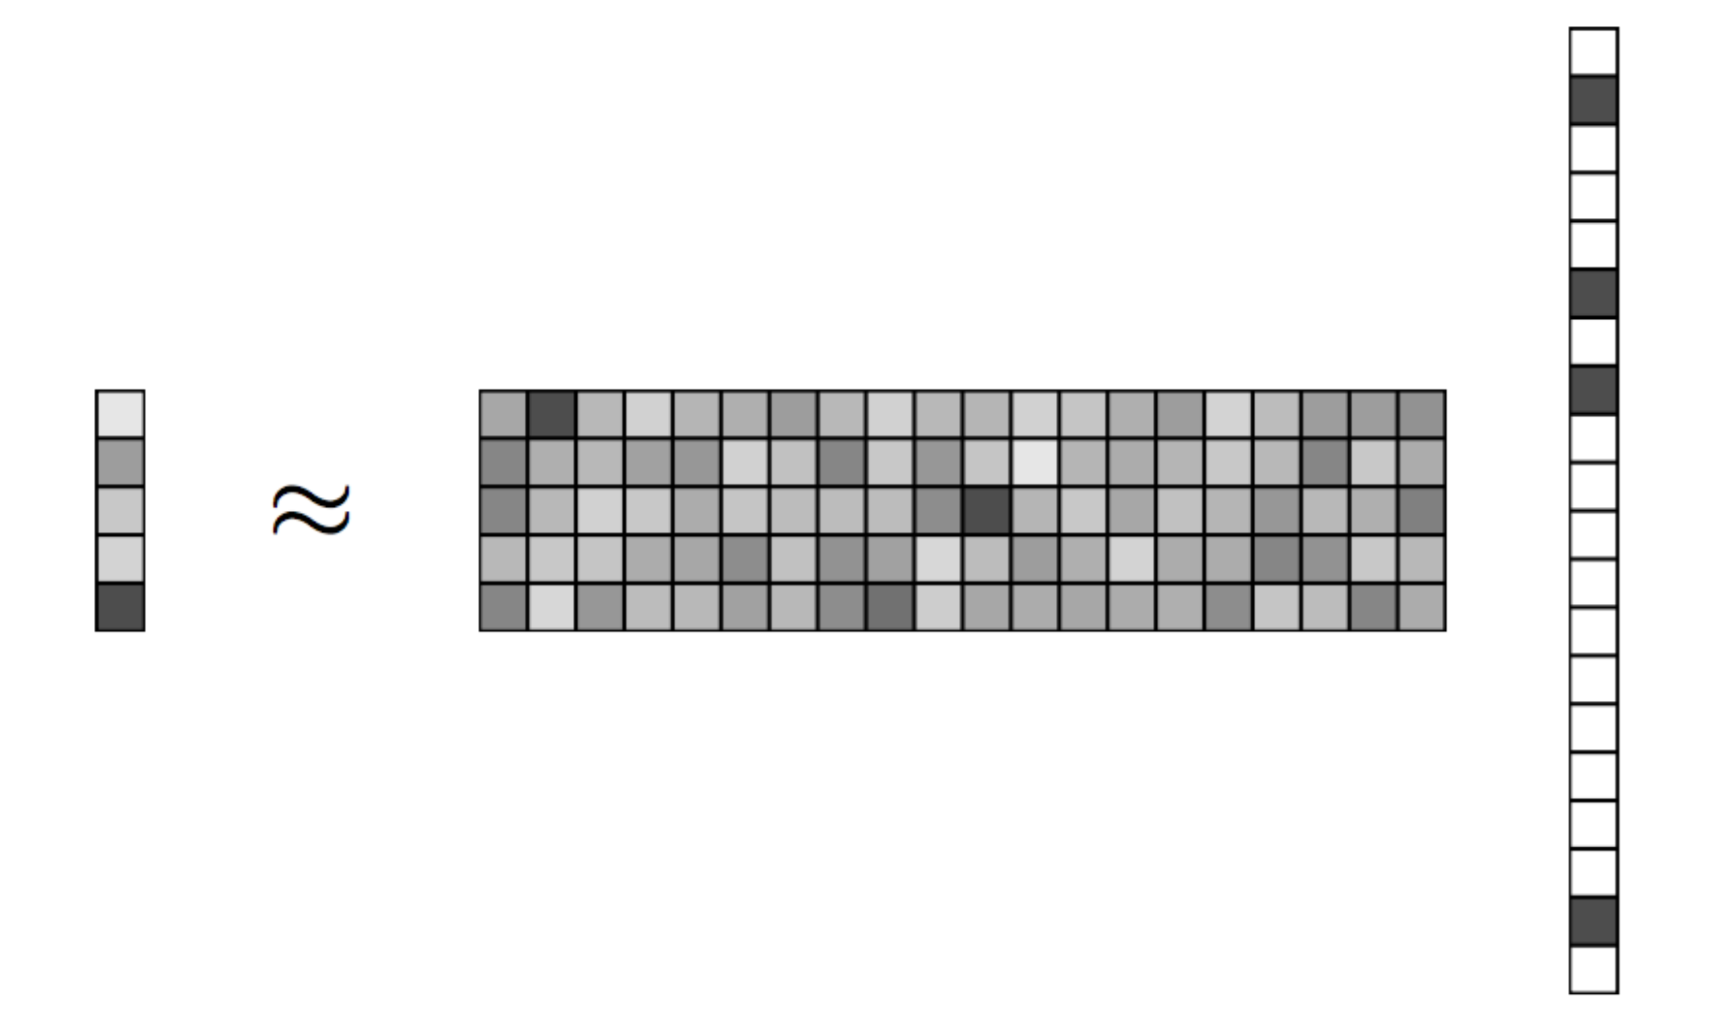
\includegraphics[width=0.6\linewidth]{Screenshot_1.png}
\caption{Разреженная линейная регрессия $Z\approx X\alpha$}
\end{figure}

\begin{definition}
\label{L1}
$L_1$~-- регуляризацией называется добавление дополнительного слагаемого $\sum\limits_{i = 1}^n |x_i|$, и исходная задача принимает вид: 
\[
\min\limits_{x}(f(x) + \lambda \sum\limits_{i = 1}^n|x_i|)
\]
\end{definition}

\section{Причем тут субмодулярность?}

Стоит отметить, что в общем случае коэффициент детерминации $R^2_{Z, S}$ не является субмодулярной функцией. В то же время исследуемые нами алгоритмы были хорошо изучены применительно к оптимизации субмодулярных функций. 

Именно по этой причине в рассмотрение вводится понятие коэффициента субмодулярности, с помощью которого можно получить новые оценки на точность аппроксимации несубмодулярной функции $R^2_{Z, S}$ алгоритмами прямой регрессии и ортогонального согласованного преследования.

Рассмотрим, каким будет коэффициент субмодулярности для функции $R^2$.
\[\gamma_{U, k}=\min_{\substack{L \subseteq U\\ S:|S| \leq k \\ S \cap L=\varnothing}} \frac{\sum_{i \in S}\left(R_{Z, L \cup\left\{X_{i}\right\}}^{2}-R_{Z, L}^{2}\right)}{R_{Z, S \cup L}^{2}-R_{Z, L}^{2}}=\min_{\substack{L \subseteq U\\ S:|S| \leq k \\ S \cap L=\varnothing}} \frac{\left(\mathbf{b}_{S}^{L}\right)^{T} \mathbf{b}_{S}^{L}}{\left(\mathbf{b}_{S}^{L}\right)^{T}\left(C_{S}^{L}\right)^{-1} \mathbf{b}_{S}^{L}},\]

где $C^L$ и $\mathbf{b}^L$ -- нормированные матрица ковариаций и вектор ковариаций для множества $\left\{\operatorname{Res}\left(X_{1}, L\right), \operatorname{Res}\left(X_{2}, L\right), \ldots, \operatorname{Res}\left(X_{n}, L\right)\right\}$.\\

Приведем следующую лемму для иллюстрации связи коэффициента субмодулярности с субмодулярностью функции.(Доказательство приведено в статье~\cite{das2011submodular})
\newtheorem{lemma}{Лемма}
\begin{lemma}
Функция $f$ субмодулярна тогда и только тогда, когда
\[\forall~U, k \hookrightarrow \gamma_{U, k} \geqslant 1\]
\end{lemma}

Введем обозначение 
\[\lambda_{\min }(C, k)=\min _{S:|S|=k} \lambda_{\min }\left(C_{S}\right)~.\]

Сформулируем следующее утверждение, содержащее спектральную оценку снизу для величины $\gamma_{U, k}$ (доказательство приведено в статье~\cite{das2011submodular}).

\begin{lemma}
\[\gamma_{U, k} \geq \lambda_{\min }(C, k+|U|) \geq \lambda_{\min }(C)\]
\end{lemma}


Для того, чтобы понять, какие оценки на аппроксимацию $R^2$ существуют, нам необходимо разобраться в устройстве изучаемых алгоритмов.

Следующим шагом опишем принцип работы рассматриваемых в работе алгоритмов, после чего приведем теоретические оценки точности их работы.
% дописать теорию для ограничений

\section{Методы}
\label{S:3}
В общем случае комбинаторная задача выбора оптимального $k$-подмножества является NP-сложной \cite{das2011submodular}. Таким образом, не существует алгоритма, способного решить такую задачу за полиномиальное время для всех входных данных. По этой причине для решения чаще всего используются два подхода: жадные алгоритмы \cite{miller2002subset, tropp2004greed, gilbert2003approximation} и выпуклые релаксационные схемы \cite{obozinski2012convex, tibshirani1996regression, candes2006stable}. Для нашей формулировки недостаток методов выпуклой релаксации заключаются в том, что они не обеспечивают явного контроля над целевым уровнем разреженности $k$.\\

Более простой и интуитивно понятный подход, широко используемый на практике для решения задач выбора оптимального подмножества (например, он интегрирован во все пакеты коммерческой статистики), заключается в использовании жадных алгоритмов, которые итеративно добавляют (или удаляют) величины $X_i$ в текущее оптимальное подмножество на основе меры соответствия их комбинации с $Z$.\\

В этой работе будут рассмотрены следующие жадные алгоритмы: Прямая Регрессия (Forward Regression) \cite{miller2002subset}, Метод Ортогонального Согласованного Преследования (Orthogonal Matching Pursuit)\cite{tropp2004greed}, Забывчивый Жадный Алгоритм (Oblivious greedy algorithm), также будет рассмотрена $L_1$~-- регуляризация.

\subsection{Forward Regression (Прямая регрессия)}
Данный алгоритм для задачи $Subset Selection$ выбирает множество $S$ размера $k$, искомое в задаче. 

\begin{algorithm}%[t!]
\caption{Forward Regression}\label{algo::fg1}
\begin{algorithmic}[1]
\Require $k \in \mathbb{N}$
\State $i := 0$;
\State $S := \emptyset$;
\While{$i < k$}
\State Выбирается случайная величина $X_m \in V \backslash S$ максимизирующая $R_{Z, S + \{X_m\}}^{2}$;
\State $S \gets S + \{X_m\}$;
\State $i \gets i + i$;
\EndWhile
\end{algorithmic}
\end{algorithm}

\subsection{Orthogonal Matching Pursuit (Метод ортогонального согласованного преследования)}
Данный алгоритм для задачи $Subset Selection$ выбирает множество $S$ размера $k$, искомое в задаче. 

\begin{algorithm}%[t!]
\caption{Orthogonal Matching Pursuit}\label{algo::fg2}
\begin{algorithmic}[1]
\Require $k \in \mathbb{N}$
\State $i := 0$;
\State $S := \emptyset$;
\While{$i < k$}
\State Выбирается случайная величина $X_m \in V \backslash S$ максимизирующая $|Cov(Res(Z, S_i), X_m)|$;
\State $S \gets S + \{X_m\}$;
\State $i \gets i + i$;
\EndWhile
\end{algorithmic}
\end{algorithm}


\subsection{Oblivious greedy algorithm}
Выбирается $k$ случайных величин $X_i$ с наибольшими значениями $\mathbf{b_i}$.\\

Данный алгоритм является самым тривиальным из исследуемых, так как в его работе вообще не используется матрица ковариаций $C$.

\subsection{$L_1$~-- регуляризация}
В описанном ранее методе (\ref{L1}) подбирается такой минимальный коэффициент $\lambda$, чтобы не более чем $k$ координат вектора $\alpha$ оказались по модулю больше некоторого малого заданного $\varepsilon$, соответствующие им признаки образуют искомое множество. Это делается для контроля количества значимых признаков, т.е. размера искомого множества.

\section{Анализ работы алгоритмов}
В этой секции мы оценим сходимость описанных выше алгоритмов. Введем величину $OPT=\max_{S:|S|=k} R_{Z, S}^{2}$ для обозначения оптимального значения $R^2$, достигаемого для любого подмножества размера $k$. 
\subsection{Forward Regression (Метод прямой регрессии)}
Для оптимального подмножества, выбранного в результате работы алгоритма прямой регрессии, введем обозначение $S^{FR}$. Основные результаты оценки работы метода приведены в следующей теореме.
\begin{theorem}[Оценки на множество $S^{FR}$\cite{das2011submodular}]
Для подмножества $S^{FR}$, выбранного методом прямой регрессии, справедливы следующие оценки:
\begin{equation}\begin{aligned}
R_{Z, S^{F R}}^{2} & \geq\left(1-e^{-\gamma_{S^{F R}, k}}\right) \cdot OPT \\
& \geq\left(1-e^{-\lambda_{\min }(C, 2 k)}\right) \cdot OPT \\
& \geq\left(1-e^{-\lambda_{\min }(C, k)}\right) \cdot \Theta\left(\left(\frac{1}{2}\right)^{1 / \lambda_{\min }(C, k)}\right) \cdot OPT
\end{aligned}\end{equation}
\end{theorem}
\subsection{Orthogonal Matching Pursuit (Метод ортогонального согласованного преследования)}
Следующий в рассмотрении алгоритм -- метод ортогонального согласованного преследования, часто используемый в обработке сигналов. Аналогично прошлому пункту, введем обозначение $S^{OMP}$. \\

Перед введением основной теоремы для текущего метода рассмотрим следующую лемму.
\begin{lemma}
Пусть $A\in\mathbb{R}^{(n+1)\times(n+1)}$ -- матрица ковариаций между случайными величинами $Z, X_1, \dots, X_n$. Тогда 
$$\mathbb{D}\left(\operatorname{Res}\left(Z,\left\{X_{1}, \ldots, X_{n}\right\}\right)\right) \geq \lambda_{\min }(A)$$
\end{lemma}
\begin{proof}
Напомним, что 
$\operatorname{Res}(Z, S)=Z-\sum\limits_{i \in S} \alpha_{i} X_{i}$. Обозначим $\mathbf{Y}= (Z, X_1, \dots, X_n)^\top $Рассмотрим данную матрицу 
$$A=\operatorname{cov}(\mathbf{Y})=\mathbb{E}\left[\mathbf{Y Y}^{\top}\right]-\mathbb{E}[\mathbf{Y}] \cdot \mathbb{E}\left[\mathbf{Y}^{\top}\right]=\left(\begin{array}{ll}
1 & \mathbf{b}^{T} \\
\mathbf{b} & C
\end{array}\right).$$
Для всякой матрицы $M$ будем обозначать как $M[i,j]$ подматрицу, полученной из нее удалением $i$-ой строки и $j$-го столбца. Пользуясь этим обозначением, распишем детерминант матрицы $A$ по первой строке:

\begin{equation}\begin{aligned}
\operatorname{det}(A) &=\sum_{j=1}^{n+1}(-1)^{1+j} a_{1, j} \operatorname{det}(A[1, j]) \\
&=\operatorname{det}(C)+\sum_{j=1}^{n}(-1)^{j} b_{j} \operatorname{det}(A[1, j+1]) \\
&=\operatorname{det}(C)+\sum_{j=1}^{n}(-1)^{j} b_{j} \sum_{i=1}^{n}(-1)^{i+1} b_{i} \operatorname{det}(C[i, j]) \\
&=\operatorname{det}(C)-\sum_{j=1}^{n} \sum_{i=1}^{n}(-1)^{i+j} b_{i} b_{j} \operatorname{det}(C[i, j]) \\
&=\operatorname{det}(C)\left(1-\mathbf{b}^{T} C^{-1} \mathbf{b}\right)
\end{aligned}\end{equation}

Таким образом, имеем $\dfrac{\operatorname{det}(A)}{\operatorname{det}(C)}=1-\mathbf{b}^{T} C^{-1} \mathbf{b}$.\\

Рассмотрим теперь дисперсию 
\[\mathbb{D}\operatorname{Res}(Z, \mathbf{X})=\mathbb{D}(Z-\sum\limits_{i \in S} \alpha_{i} X_{i})=1-\mathbb{D}(\sum\limits_{i \in S} \alpha_{i} X_{i})= 1-\mathbf{b}^{T} C^{-1} \mathbf{b}=\dfrac{\operatorname{det}(A)}{\operatorname{det}(C)}.\]
Так как
$\operatorname{det}(A)=\prod_{i=1}^{n+1} \lambda_{i}^{A}$ и $\operatorname{det}(C)=\prod_{i=1}^{n} \lambda_{i}^{C}$, а также, что по теореме Коши о переплетении \cite{gowda2011cauchy} $\lambda_{1}^{A} \leq \lambda_{1}^{C} \leq \lambda_{2}^{A} \leq \lambda_{2}^{C} \leq \ldots \leq \lambda_{n+1}^{A}$, получаем 
\[\mathbb{D}\operatorname{Res}(Z, \mathbf{X})=\frac{\operatorname{det}(A)}{\operatorname{det}(C)} \geq \lambda_{1}^{4},\]
лемма доказана.
\end{proof}

Теперь сформулируем известные оценки точности метода OMP.

\begin{theorem}[Оценки на множество $S^{OMP}$ \cite{das2011submodular}]
Подмножество $S^{OMP}$, выбранное алгоритмом OMP, имеет следующие оценки аппроксимации коэффициента детерминации:
\begin{equation}\begin{aligned}
R_{Z, S^{O M P}}^{2} & \geq\left(1-e^{-\left(\gamma_{S} O u_{, k} \cdot \lambda_{\min }(C, 2 k)\right)}\right) \cdot OPT \\
& \geq\left(1-e^{-\lambda_{\min }(C, 2 k)^{2}}\right) \cdot OPT \\
& \geq\left(1-e^{-\lambda_{\min }(C, k)^{2}}\right) \cdot \Theta\left(\left(\frac{1}{2}\right)^{1 / \lambda_{\min }(C, k)}\right) \cdot OPT
\end{aligned}\end{equation}

\end{theorem}

\subsection{Oblivious Greedy Algorithm}
\begin{theorem}[Оценка на множество $S^{Oblivious}$ \cite{das2011submodular}]
Пусть подмножество $S^{Oblivious}$ было выбрано в результате работы забывчивого жадного алгоритма. Тогда справедливы следующие оценки аппроксимации коэффициента детерминации:
\begin{equation}R_{Z, S^{O B L}}^{2} \geq \frac{\gamma_{0, k}}{\lambda_{\max }(C, k)} \cdot O P T \geq \frac{\lambda_{\min }(C, k)}{\lambda_{\max }(C, k)} \cdot O P T\end{equation}
\end{theorem}
\section{Эксперименты}
\label{S:4}

\begin{figure}[H]
    \begin{minipage}{.49\textwidth}
        \centering
        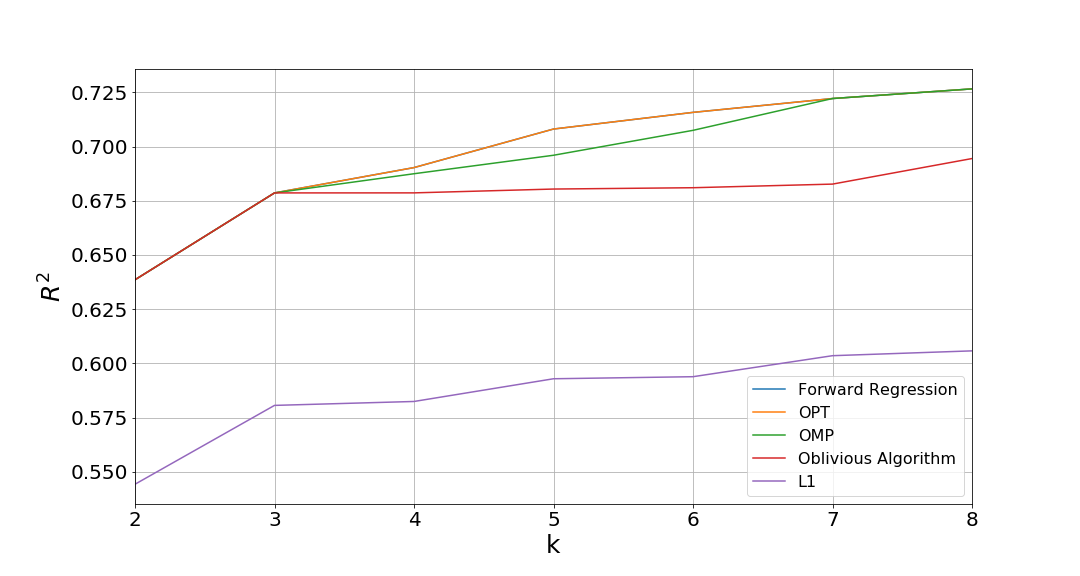
\includegraphics[width=1.1\linewidth]{img/boston_housing.png}
        \caption{Сравнение результатов работы алгоритмов на данных Boston Housing}
    \end{minipage}
    \begin{minipage}{.49\textwidth}
        \centering
        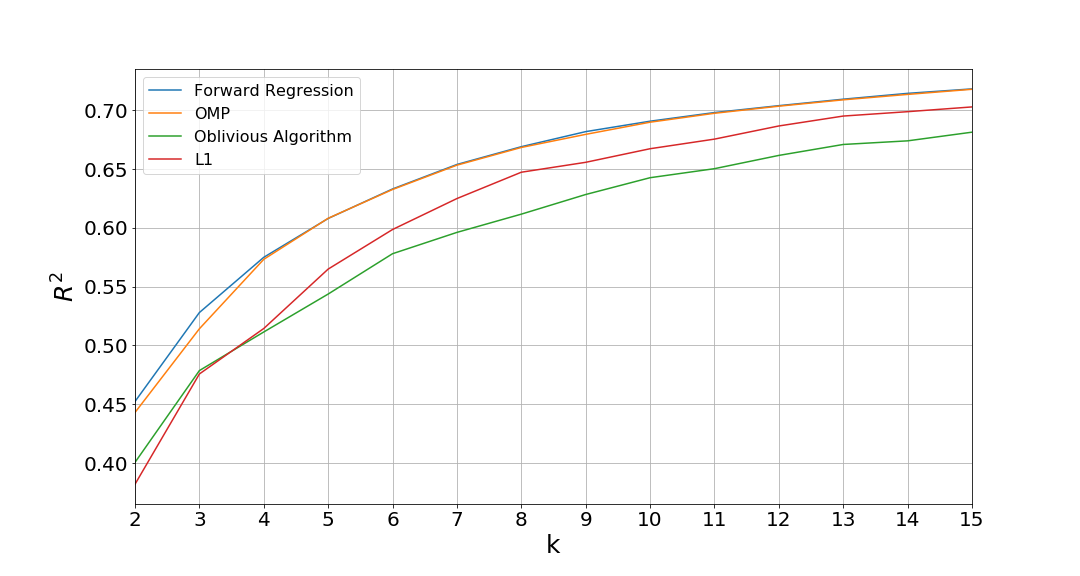
\includegraphics[width=1.1\linewidth]{img/sythetic_data.png}
        \caption{Сравнение результатов работы алгоритмов на синтетических данных}
    \end{minipage}
\end{figure}

Исследуемые методы были проверены на двух наборах данных: Boston Housing и синтетических данных ($X_i$ сгенерированы из многомерного нормального распределения с матрицей ковариации $C$, близкой к вырожденной, и $Z = \sum\limits_{i = 1}^n \alpha_i X_i + \varepsilon$, где $\varepsilon$ - нормально распределенная случайная величина). Из графиков видно, что наилучший результат показывает метод Прямой Регрессии (Forward Regression), достаточной близкий результат у метода Ортогонального Согласованного Преследования (Orthogonal Matching Pursuit), а Забывчивый жадный алгоритм (Oblivious greedy Algorithm) показывает существенно меньший результат. На реальных данных хуже всего себя показывает $L_1$~-- регуляризация. Важно отметить, что Например, для $k = 5$ и $k = 8$ на данных Boston Housing были достигнуты следующие результаты: 
\begin{center}
    \begin{tabular}{ |c|c|c|c|c| } 
        \hline
          & Forward  & OMP & Oblivious& $L_1$ \\ 
          &  Regression & & Algorithm & \\ 
         \hline
         $k = 5$ & 0.71 & 0.70 & 0.68 & 0.59\\ 
         \hline
         $k = 8$ & 0.73 & 0.73 & 0.69& 0.61\\ 
         \hline
    \end{tabular}
\end{center}


\section{Выводы}
\begin{itemize}
    \item Наилучший результат на двух наборах данных показывает метод Прямой Регрессии (Forward Regression).
    \item Забывчивый жадный Алгоритм (Oblivious greedy Algorithm) и $L_1$-регуляризация показывают результаты, существенно уступающие Прямой Регрессии (Forward Regression) и  Ортогональному Согласованному Преследованию (Orthogonal Matching Pursuit).
\end{itemize}

\section{Заключение}

В данной статье были рассмотрены такие задачи, как Выбор оптимального подмножества и Выбор оптимального словаря. Эти задачи были рассмотрены в контексте отбора признаков. Для их решения были подобраны жадные алгоритмы: Прямая Регрессия (Forward Regression), Ортогональное Согласованное Преследование (Orthogonal Matching Pursuit), Забывчивый жадный алгоритм (Oblivious greedy Algorithm). Так же была рассмотрена $L_1$-регуляризация (Lasso Regression). Наилучший коэффициент детерминации лучший результат показали Прямая Регрессия и Ортогональное Согласованное Преследование на реальных и синтетических данных. Соответственно худший результат показали Забывчивый жадный алгоритм и $L_1$-регуляризация. Для данных жадных алгоритмов были подтверждены теоретические оценки на точность аппроксимации оптимального $OPT$. 
\section{Направление исследования в будущем}
В дальнейших исследованиях планируется исследовать возможность решения схожей задачи с помощью эвристик, например Прямо-обратная Регрессия (Forward-backward Regression), Поиск в Ширину (Breadth-first Search), Поиск в Глубину (Depth-first Search), и Генетические алгоритмы (Genetic Algorithm)~\cite{vorontcov2007lectures}.



% \section{Список литературы}

% \newpage
\bibliographystyle{unsrt}
\bibliography{sample.bib}
\end{document}

%%
%% End of file `elsarticle-template-1-num.tex'.